\documentclass[11pt,compress,t,notes=noshow, xcolor=table]{beamer}
\usepackage[]{graphicx}\usepackage[]{color}
% maxwidth is the original width if it is less than linewidth
% otherwise use linewidth (to make sure the graphics do not exceed the margin)
\makeatletter
\def\maxwidth{ %
  \ifdim\Gin@nat@width>\linewidth
    \linewidth
  \else
    \Gin@nat@width
  \fi
}
\makeatother

\definecolor{fgcolor}{rgb}{0.345, 0.345, 0.345}
\newcommand{\hlnum}[1]{\textcolor[rgb]{0.686,0.059,0.569}{#1}}%
\newcommand{\hlstr}[1]{\textcolor[rgb]{0.192,0.494,0.8}{#1}}%
\newcommand{\hlcom}[1]{\textcolor[rgb]{0.678,0.584,0.686}{\textit{#1}}}%
\newcommand{\hlopt}[1]{\textcolor[rgb]{0,0,0}{#1}}%
\newcommand{\hlstd}[1]{\textcolor[rgb]{0.345,0.345,0.345}{#1}}%
\newcommand{\hlkwa}[1]{\textcolor[rgb]{0.161,0.373,0.58}{\textbf{#1}}}%
\newcommand{\hlkwb}[1]{\textcolor[rgb]{0.69,0.353,0.396}{#1}}%
\newcommand{\hlkwc}[1]{\textcolor[rgb]{0.333,0.667,0.333}{#1}}%
\newcommand{\hlkwd}[1]{\textcolor[rgb]{0.737,0.353,0.396}{\textbf{#1}}}%
\let\hlipl\hlkwb

\usepackage{framed}
\makeatletter
\newenvironment{kframe}{%
 \def\at@end@of@kframe{}%
 \ifinner\ifhmode%
  \def\at@end@of@kframe{\end{minipage}}%
  \begin{minipage}{\columnwidth}%
 \fi\fi%
 \def\FrameCommand##1{\hskip\@totalleftmargin \hskip-\fboxsep
 \colorbox{shadecolor}{##1}\hskip-\fboxsep
     % There is no \\@totalrightmargin, so:
     \hskip-\linewidth \hskip-\@totalleftmargin \hskip\columnwidth}%
 \MakeFramed {\advance\hsize-\width
   \@totalleftmargin\z@ \linewidth\hsize
   \@setminipage}}%
 {\par\unskip\endMakeFramed%
 \at@end@of@kframe}
\makeatother

\definecolor{shadecolor}{rgb}{.97, .97, .97}
\definecolor{messagecolor}{rgb}{0, 0, 0}
\definecolor{warningcolor}{rgb}{1, 0, 1}
\definecolor{errorcolor}{rgb}{1, 0, 0}
\newenvironment{knitrout}{}{} % an empty environment to be redefined in TeX

\usepackage{alltt}
\newcommand{\SweaveOpts}[1]{}  % do not interfere with LaTeX
\newcommand{\SweaveInput}[1]{} % because they are not real TeX commands
\newcommand{\Sexpr}[1]{}       % will only be parsed by R
\newcommand{\xmark}{\ding{55}}%


\usepackage[english]{babel}
\usepackage[utf8]{inputenc}

\usepackage{dsfont}
\usepackage{verbatim}
\usepackage{amsmath}
\usepackage{amsfonts}
\usepackage{amssymb}
\usepackage{bm}
\usepackage{csquotes}
\usepackage{multirow}
\usepackage{longtable}
\usepackage{booktabs}
\usepackage{enumerate}
\usepackage[absolute,overlay]{textpos}
\usepackage{psfrag}
\usepackage{algorithm}
\usepackage{algpseudocode}
\usepackage{eqnarray}
\usepackage{arydshln}
\usepackage{tabularx}
\usepackage{placeins}
\usepackage{tikz}
\usepackage{setspace}
\usepackage{colortbl}
\usepackage{mathtools}
\usepackage{wrapfig}
\usepackage{bm}
\usepackage{amsmath}
\usepackage{pifont}
\usepackage{xcolor} %colored math symbols

\usetikzlibrary{shapes,arrows,automata,positioning,calc,chains,trees, shadows}
\tikzset{
  %Define standard arrow tip
  >=stealth',
  %Define style for boxes
  punkt/.style={
    rectangle,
    rounded corners,
    draw=black, very thick,
    text width=6.5em,
    minimum height=2em,
    text centered},
  % Define arrow style
  pil/.style={
    ->,
    thick,
    shorten <=2pt,
    shorten >=2pt,}
}

\usepackage{subfig}

% Defines macros and environments
\usepackage{../../style/lmu-lecture}


\let\code=\texttt
\let\proglang=\textsf

\setkeys{Gin}{width=0.9\textwidth}

\setbeamertemplate{frametitle}{\expandafter\uppercase\expandafter\insertframetitle}

\usepackage{bbm}
% basic latex stuff
\newcommand{\pkg}[1]{{\fontseries{b}\selectfont #1}} %fontstyle for R packages
\newcommand{\lz}{\vspace{0.5cm}} %vertical space
\newcommand{\dlz}{\vspace{1cm}} %double vertical space
\newcommand{\oneliner}[1] % Oneliner for important statements
{\begin{block}{}\begin{center}\begin{Large}#1\end{Large}\end{center}\end{block}}


%new environments
\newenvironment{vbframe}  %frame with breaks and verbatim
{
 \begin{frame}[containsverbatim,allowframebreaks]
}
{
\end{frame}
}

\newenvironment{vframe}  %frame with verbatim without breaks (to avoid numbering one slided frames)
{
 \begin{frame}[containsverbatim]
}
{
\end{frame}
}

\newenvironment{blocki}[1]   % itemize block
{
 \begin{block}{#1}\begin{itemize}
}
{
\end{itemize}\end{block}
}

\newenvironment{fragileframe}[2]{  %fragile frame with framebreaks
\begin{frame}[allowframebreaks, fragile, environment = fragileframe]
\frametitle{#1}
#2}
{\end{frame}}


\newcommand{\myframe}[2]{  %short for frame with framebreaks
\begin{frame}[allowframebreaks]
\frametitle{#1}
#2
\end{frame}}

\newcommand{\remark}[1]{
  \textbf{Remark:} #1
}


\newenvironment{deleteframe}
{
\begingroup
\usebackgroundtemplate{
\includegraphics[width=\paperwidth,height=\paperheight]{../style/color/red.png}}
 \begin{frame}
}
{
\end{frame}
\endgroup
}
\newenvironment{simplifyframe}
{
\begingroup
\usebackgroundtemplate{
\includegraphics[width=\paperwidth,height=\paperheight]{../style/color/yellow.png}}
 \begin{frame}
}
{
\end{frame}
\endgroup
}\newenvironment{draftframe}
{
\begingroup
\usebackgroundtemplate{
\includegraphics[width=\paperwidth,height=\paperheight]{../style/color/green.jpg}}
 \begin{frame}
}
{
\end{frame}
\endgroup
}
% https://tex.stackexchange.com/a/261480: textcolor that works in mathmode
\makeatletter
\renewcommand*{\@textcolor}[3]{%
  \protect\leavevmode
  \begingroup
    \color#1{#2}#3%
  \endgroup
}
\makeatother


\input{../../latex-math/basic-math}
\input{../../latex-math/basic-ml}
\input{../../latex-math/ml-nn}

\newcommand{\titlefigure}{figure/loss_surface.png}
\newcommand{\learninggoals}{
  \item Gradient descent
  \item Stochastic gradient descent
  \item Minibatch gradient descent
  \item Learning rates and (S)GD specifics
}

\title{Deep Learning}
\date{}

\begin{document}

\lecturechapter{Basic Training}
\lecture{I2DL}
%%%%%%%%%%%%%%%%%%%%%%%%%%%%%%%%%%%%%%%%%%%%%%%%%%%%%%%%%%%%%%%%%%

\begin{vbframe}{Training Neural Networks}
\lz
Training of neural nets is composed of two iterative steps:
\lz
\begin{enumerate}
\item \textbf{Forward pass:} The information of the inputs flows through the model to produce a prediction. Based on this prediction, the empirical risk is computed.
\lz
\item \textbf{Backward pass:} The information of the prediction error flows backward through the network to update the weights in a way that the error reduces.
\end{enumerate}
\lz

\textbf{Recall:} The error is calculated via a loss function $L(y, f(\xv, \thetab))$, where $y$ and $f(\xv, \thetab)$ are the true target and the network outcome, respectively.
\framebreak
%%%%%%%%%%%%%%%%%%%%%%%%%%%%%%%%%%%%%%%%%%%%%%%%%%%%%%%%%%%%%%%%%%

\lz
\lz
\begin{itemize}
\item For regression, the L2 loss is typically used:
$$\Lxy = \frac{1}{2}(y - \fx)^2$$
\item For binary classification, the binary cross entropy:
$$\Lxy = - (y \log \fx + (1 - y) \log(1 - \fx))$$
\end{itemize}
\lz
\textbf{Note:} Evaluating the loss on the data, the \textbf{empirical risk function} is computed:
$$\riske = \frac{1}{n} \sumin \Lxyi$$
\begin{itemize}
 \item To minimize the empirical risk, the \textbf{gradient descent} (GD) method can be used.
\end{itemize}
\end{vbframe}

%%%%%%%%%%%%%%%%%%%%%%%%%%%%%%%%%%%%%%%%%%%%%%%%%%%%%%%%%%%%%%%%%%

\begin{vbframe}{Gradient descent}
  \begin{itemize}
    \item Let $\riske: \R^m \to \R$ be an arbitrary, differentiable, unrestricted function (of $\thetab \in \R^m$). \\
    \begin{footnotesize}
    In the context of deep learning, $\riske$ represents the empirical risk function and $\thetab$ represents the weights (and biases) of the network. For simplification, we assume $\bm{\theta} = (\theta_1, ..., \theta_m)$. 
    \end{footnotesize}
    \item We want to minimize this function by gradient descent (GD). 
    \item The negative gradient 
    $$
    - \mathbf{g} = - \nabla \riske(\thetab) = - \left(\frac{\partial \riske}{\partial \theta_1}, \ldots, \frac{\partial \riske}{\partial \theta_m}\right)^\top
    $$ 
    points in the direction of the \textbf{steepest descent}, since $\nabla \riske$ always points in the direction of the steepest ascent.
  \end{itemize}

    \framebreak

  \begin{itemize}
    \item \enquote{Standing} at a point $\thetab^{[t]}$ during minimization, we improve by performing the following update: 
    $$
      \thetab^{[t + 1 ]}  = \thetab^{[t]} - \alpha \nabla \riske\left(\thetab^{[t]}\right),
    $$
    which implies (for sufficiently small $\alpha$),
    $$
    \riske(\bm{\thetab}^{[t+1]}) \leq \riske(\bm{\thetab}^{[t]})
    $$
    \item $\alpha$ determines the length of the step and is called \textbf{step size} or, in risk minimization, \textbf{learning rate}.
  \end{itemize}

\end{vbframe} 

%%%%%%%%%%%%%%%%%%%%%%%%%%%%%%%%%%%%%%%%%%%%%%%%%%%%%%%%%%%%%%%%%%

\begin{vbframe}{Example: Gradient descent}
\begin{center}
 $\riske(\theta_1, \theta_2) = -\sin(\theta_1) \cdot \frac{1}{2\pi} \exp\left( (\theta_2 - \pi / 2)^2 \right)$
\begin{figure}
\centering
\scalebox{0.9}{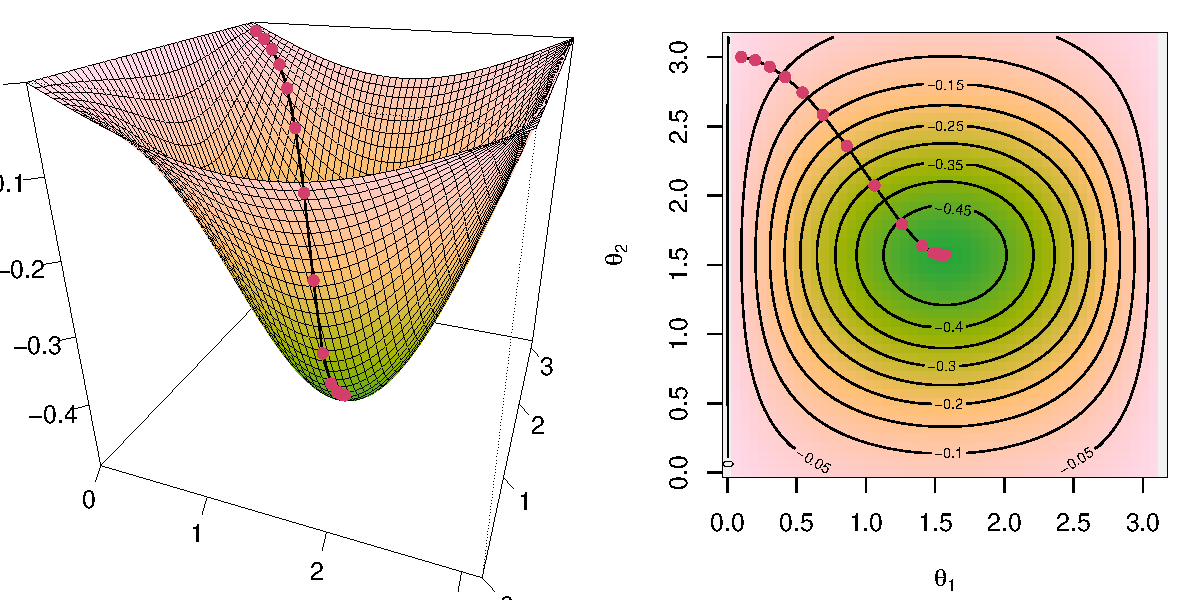
\includegraphics{figure_man/hill.pdf}}
\end{figure}
\vspace{0.5 cm}
"Walking down the hill, towards the valley."
\end{center}
\end{vbframe}
%%%%%%%%%%%%%%%%%%%%%%%%%%%%%%%%%%%%%%%%%%%%%%%%%%%%%%%%%%%%%%%%%%

\begin{vbframe}{Gradient Descent and Optimality}

\begin{minipage}{0.45\textwidth}
    \begin{small}
    \begin{itemize}
      \item GD is a greedy algorithm: In every iteration, it makes locally optimal moves.
      \vspace*{2mm}
      \item If $\riske(\thetab)$ is \textbf{convex} and \textbf{differentiable}, and its gradient is Lipschitz continuous, GD is guaranteed to converge to the global minimum (for small enough step-size).  
      \vspace*{2mm}
    \item However, if $\riske(\thetab)$ has multiple local optima and/or saddle points, GD might only converge to a stationary point (other than the global optimum), depending on the starting point. 
    \end{itemize}
    \end{small}
  \end{minipage}\hfill
  \begin{minipage}{0.5\textwidth}
    \begin{figure}
      \centering
        \scalebox{1}{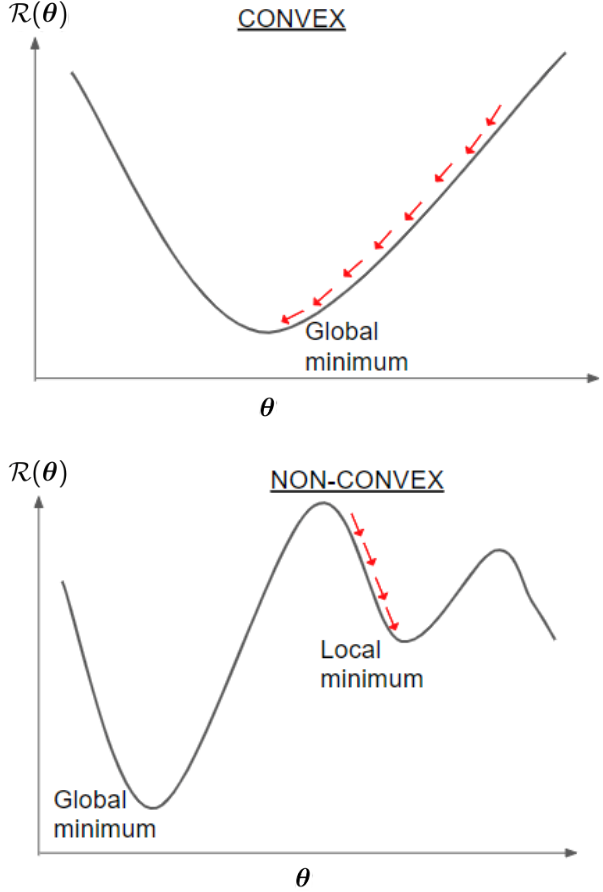
\includegraphics{figure/gdes3.png}}
    \end{figure}
  \end{minipage}  

  \framebreak 

  \textbf{Note: } It might not be that bad if we do not find the global optimum:  

  \begin{itemize}
    \item We do not optimize the actual quantity of interest, i.e. the (theoretical) risk, but only an approximate version, i.e. the empirical risk. 
    \item If the model class is very flexible, it might be disadvantageous to optimize too aggressively and increase the risk of overfitting. 
    \item Early-stopping the optimization might even increase generalization performance. 
  \end{itemize}

\end{vbframe}

%%%%%%%%%%%%%%%%%%%%%%%%%%%%%%%%%%%%%%%%%%%%%%%%%%%%%%%%%%%%%%%%%%

\begin{vbframe}{Learning rate}

The step-size $\alpha$ plays a key role in the convergence of the algorithm.
\lz

If the step size is too small, the training process may converge \textbf{very} slowly (see left image). If the step size is too large, the process may not converge, because it \textbf{jumps} around the optimal point (see right image).

\begin{center}
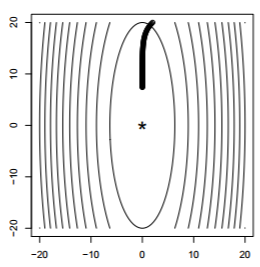
\includegraphics[width = 0.3\textwidth]{figure/stepsize_small.png}~~
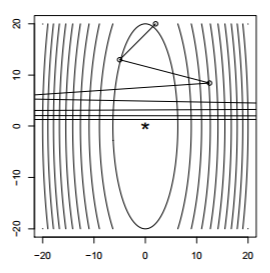
\includegraphics[width = 0.3\textwidth]{figure/stepsize_large.png}
\end{center}

\end{vbframe}

%%%%%%%%%%%%%%%%%%%%%%%%%%%%%%%%%%%%%%%%%%%%%%%%%%%%%%%%%%%%%%%%%%

\begin{vbframe}{Learning Rate}


So far we have assumed a fixed value of $\alpha$ in every iteration:

\vspace*{-0.2cm}
$$\alpha^{[t]} = \alpha \quad \forall t = {\{1, \ldots, T\}}$$

% \textbf{Konvergenz:} Es sei $f:\R^n \to \R$ konvex, differenzierbar und Liptschitz-stetig, d.h. es gibt ein $L > 0$
%
% $$
% \|\nabla f(\bm{x}) - \nabla f(\bm{y})\| \le L\|\bm{x} - \bm{y}\| \quad \text{f?r alle} x, y
%

However, it makes sense to adapt $\alpha$ in every iteration:


\vspace*{-0.1cm}
\begin{center}
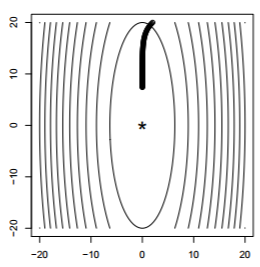
\includegraphics[width = 0.3\textwidth]{figure/stepsize_small.png} ~~~ 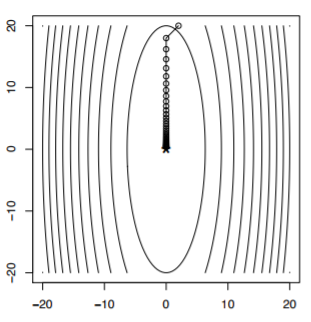
\includegraphics[width = 0.3\textwidth]{figure/stepsize_adaptive.png} \\
\end{center}
\begin{footnotesize}
Steps of gradient descent for $\riske(\thetab) = 10\,\theta_1^2 + 0.5\,\theta_2^2$. Left:  100 steps for with a fixed learning rate. Right:  40 steps with an adaptive learning rate.
\end{footnotesize}


\end{vbframe}
%%%%%%%%%%%%%%%%%%%%%%%%%%%%%%%%%%%%%%%%%%%%%%%%%%%%%%%%%%%%%%%%%%

\begin{vbframe}{Weight Initialization}
\begin{itemize}
\item The weights (and biases) of a neural network must be assigned some initial values before training can begin.
\item It’s important to initialize the weights randomly in order to "break symmetry". If two neurons (with the same activation function in a fully connected network) are connected to the same inputs and have the same initial weights, then both neurons will have the same gradient update in a given iteration and they’ll end up learning the same features.
\item Weights are typically drawn from a uniform a Gaussian distribution (both centered at 0 with a small variance).
\item Two common initialization strategies are ’Glorot initialization’ and ’He initialization’ which tune the variance of these distributions based on the topology of the network.
\end{itemize}
\end{vbframe}

%\begin{vbframe}{Weight updates with Backpropagation}
%\begin{itemize}
%\lz
%\item To update each weight $w \in \thetab$ in the network, we need their gradients w.r.t. the empirical risk.
%\lz
%\lz
%\item Since weights are stacked in layers inside the network, we need to repeatedly apply the \enquote{chain rule of calculus}. This process is called \textbf{backpropagation}.
%\lz
%\lz
%\item After obtaining the gradients, the weights can be updated by GD:
%$$\thetab^{[t + 1]} = \thetab^{[t]} - \alpha \cdot \frac{1}{n} \cdot \sumin \nabla_\theta L\left(\yi, f(\xi ~|~ \thetab^{[t]})\right)$$
%\end{itemize}
%\end{vbframe}

%%%%%%%%%%%%%%%%%%%%%%%%%%%%%%%%%%%%%%%%%%%%%%%%%%%%%%%%%%%%%%%%%%

\begin{vbframe}{Stochastic gradient descent}

Let us consider GD for empirical risk minimization. The updates are: 

$$
  \thetab^{[t + 1]} = \thetab^{[t]} - \alpha \cdot \frac{1}{n} \cdot \sumin \nabla_\theta L\left(\yi, f(\xi ~|~ \thetab^{[t]})\right)
$$


  \begin{itemize}
    \item Optimization algorithms that use the entire training set to compute updates in one huge step are called \textbf{batch} or \textbf{deterministic}. This is computationally very costly or often impossible. 
    \item \textbf{Idea:} Instead of letting the sum run over the whole dataset (\textbf{batch mode}) one can also let it run only over small subsets (\textbf{minibatches}), or only over a single example $i$. 
     \item If the index $i$ of the training example is a random variable with uniform distribution, then its expectation is the batch gradient $\nabla_\theta \risket$
    \item[$\to$] We have a \textbf{stochastic}, noisy version of the batch gradient

    \framebreak 

    \item The gradient w.r.t. a single training observation is fast to compute but not reliable. It can be used simply as a computational trick to deal with large data or to operate on real streams of online data in online learning.
    \item In contrast, the full
    batch gradient is costly (or even impossible, e.g., when data does not even fit into memory) to compute, particularly in DL, but it averages out all the noise from sub-sampling.
    \item Minibatches are in between. The batch size decides upon the compromise
    between speed and averaging (smoothing).
    \item In summary: SGD computes an unbiased estimate of the gradient by taking the average gradient over a minibatch (or one sample) to update the parameter $\thetab$ in this direction.
    % \item Optimization algorithms that use only a single example at a time are called \textbf{stochastic} or \textbf{online}. This can be used simply as a computational trick to deal with large data or to operate on real streams of online data in online learning.
% Those methods are called \textbf{minibatch} or \textbf{stochastic}.
  \end{itemize}
 
  \framebreak

%%%%%%%%%%%%%%%%%%%%%%%%%%%%%%%%%%%%%%%%%%%%%%%%%%%%%%%%%%%%%%%%%%
 
 An illustration of the SGD algorithm (to minimize the function $1.25(x_1 + 6)^2 + (x_2 - 8)^2)$.
 \begin{figure}
    \scalebox{0.8}{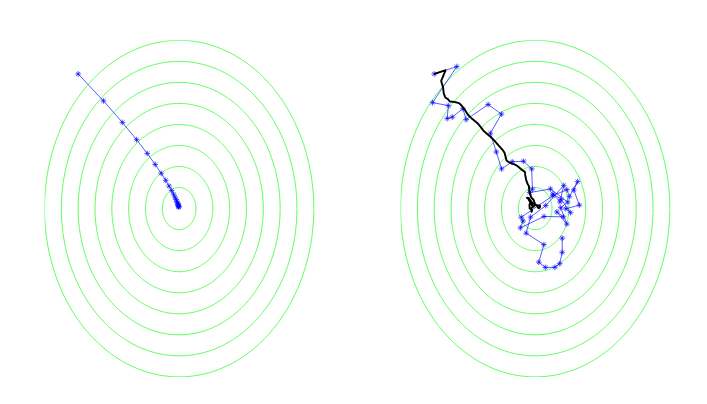
\includegraphics{figure_man/SGD.png}}
    \tiny{\\ Source : Shalev-Shwartz and  Ben-David.
Understanding machine learning: From theory to algorithms. Cambridge University Press, 2014. }
 \caption{On the left is GD and on the right is SGD. The black line depicts the averaged value of $\thetab$.}
 \end{figure}

  \end{vbframe}
  
%%%%%%%%%%%%%%%%%%%%%%%%%%%%%%%%%%%%%%%%%%%%%%%%%%%%%%%%%%%%%%%%%%

\begin{vbframe}{SGD with Momentum}
\begin{itemize}
\item While SGD remains a popular optimization strategy, learning with it can sometimes be slow.
\item Momentum is designed to accelerate learning, by accumulating an exponentially decaying moving average of past gradients.
\item Nice tool to get a feel for how momentum works: \url{https://distill.pub/2017/momentum/}
\end{itemize}
\begin{figure}
\centering
\scalebox{.55}{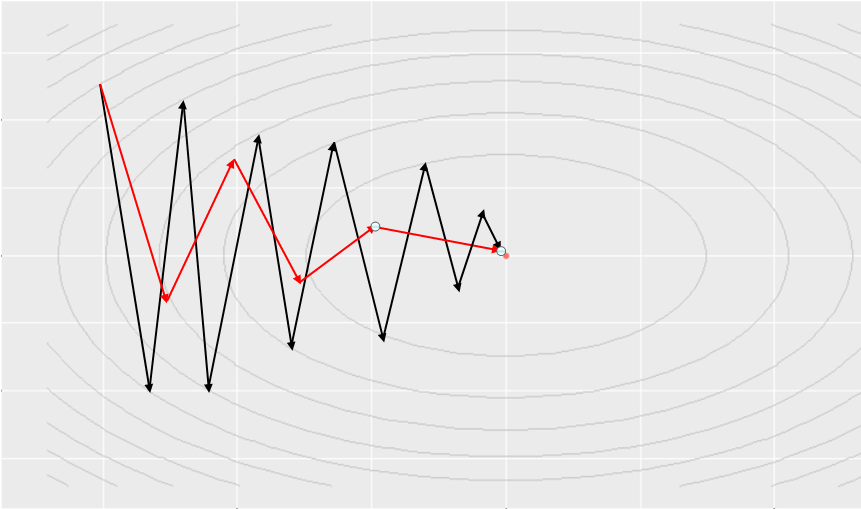
\includegraphics{figure_man/momentum.png}}
\\GD (black) versus momentum (red) when dealing with ravines
\end{figure}
\end{vbframe}

%%%%%%%%%%%%%%%%%%%%%%%%%%%%%%%%%%%%%%%%%%%%%%%%%%%%%%%%%%%%%%%%%%

\begin{vbframe}{Stochastic gradient descent}

  \begin{algorithm}[H]
  \footnotesize
    \caption{Basic SGD pseudo code}
    \begin{algorithmic}[1]
    \State Initialize parameter vector $\thetab^{[0]}$ 
    
    \State $t \leftarrow 0$
    \While{stopping criterion not met}
    \State Randomly shuffle data and partition into minibatches $J_1, ..., J_K$ of size $m$
      \For{$k\in\{1,...,K\}$} 
      \State $t \leftarrow t + 1$ 
      \State Compute gradient estimate with $J_k$: $\hat{g}^{[t]} \leftarrow \frac{1}{m} \sum_{i \in J_k} \nabla_\theta L(\yi, f(\xi ~|~ \thetab^{[t-1]})) $
      \State Apply update: $\thetab^{[t]} \leftarrow \thetab^{[t-1]} - \alpha \hat{g}^{[t]}$
      
      \EndFor
    
        
      \EndWhile
    \end{algorithmic}
  \end{algorithm}
  % \begin{itemize}
  %   \item Thus, what SGD basically does is computing an unbiased estimate of the gradient by taking the average gradients of a minibatch to update the parameter $\thetab$.
  % \end{itemize}
 
\framebreak

%%%%%%%%%%%%%%%%%%%%%%%%%%%%%%%%%%%%%%%%%%%%%%%%%%%%%%%%%%%%%%%%%%
  \begin{itemize}
    \item With minibatches of size $m$, a full pass over the training set (called an \textbf{epoch}) consists of $\frac{n}{m}$ gradient updates (\textbf{iterations}).
    \item SGD and its modifications are the most used optimization algorithms for ML in general and for deep learning in particular.
    \item SGD (with one or a few samples per batch) updates have a high variance, even though they are unbiased. 
      Because of this variance, the learning rate $\alpha$ is typically much smaller than in the full-batch scenario.
    \item SGD with minibatches reduces the variance of the parameter updates and utilizes highly optimized matrix operations to efficiently compute gradients.
   \end{itemize}
\vspace*{0.5cm}
\textbf{Note:} Sometimes, SGD with minibatches is referred to as "Minibatch gradient descent" with the term SGD being reserved for updates using a single example.

\framebreak 

%%%%%%%%%%%%%%%%%%%%%%%%%%%%%%%%%%%%%%%%%%%%%%%%%%%%%%%%%%%%%%%%%%

\vspace*{0.5cm}
  \begin{itemize}
    \item Minibatch sizes are typically between 50 and 1000.
    \item When the learning rate is slowly decreased, SGD converges to a local minimum.
    \item Recent results indicate, that SGD often leads to better generalizing models then GD, and thus may perform some kind of indirect regularization.
    \item Now we know how we can optimize/train a neural network based on the gradient, but how do we compute the gradient? We will learn more about this in the chapter on backpropagation, a method to efficiently compute gradients.
  \end{itemize}
\end{vbframe}

%%%%%%%%%%%%%%%%%%%%%%%%%%%%%%%%%%%%%%%%%%%%%%%%%%%%%%%%%%%%%%%%%%

\endlecture
\end{document}